\subsection{High-level components and their interaction}

The main software components forming the system, the interfaces provided and required from the software units, along with the relationship of necessity between components, are shown in the component diagram below [figure \ref{fig:high-lev-comp-diag}].

For a more detailed description of each component and of each interfaces, required and provided, please refer to the corresponding sections.
\begin{figure}[H]
	\centerline{
		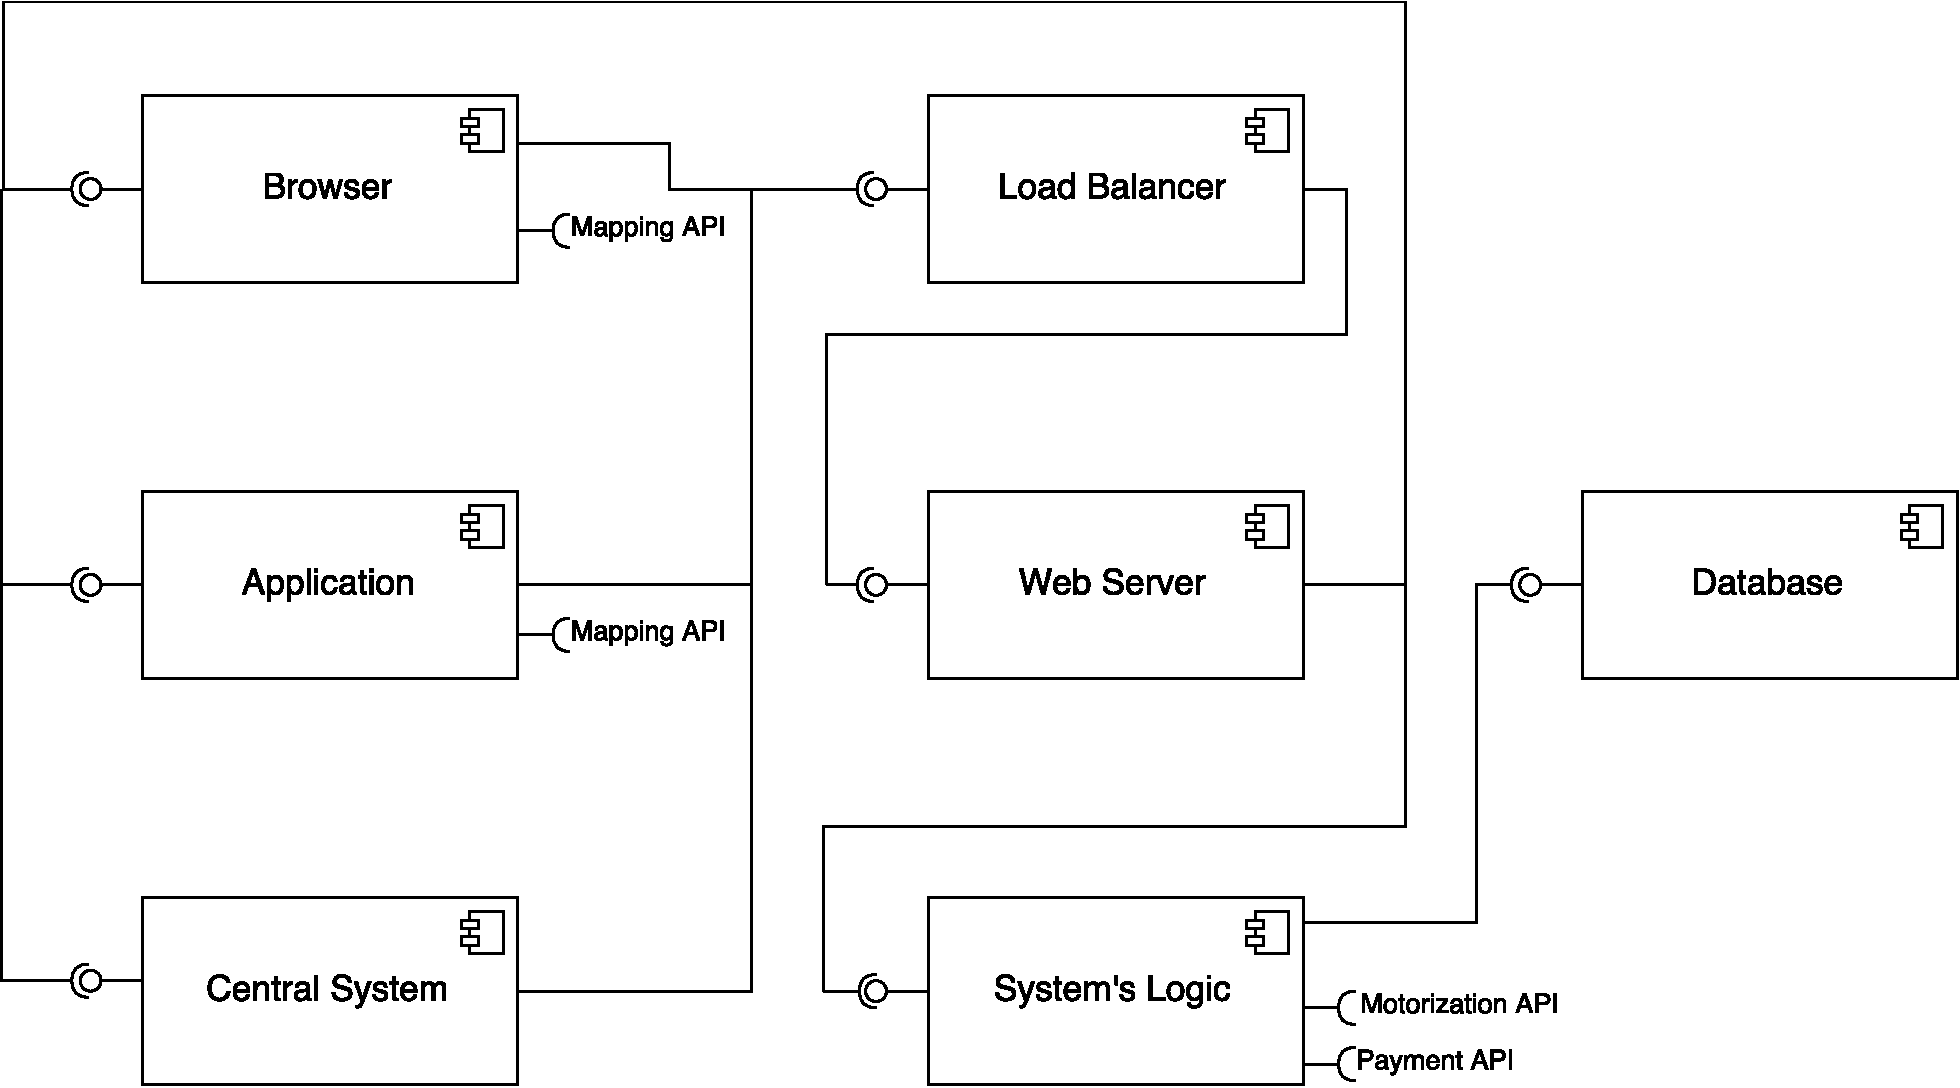
\includegraphics[width=400px]{../Datas/images/high-level-component-diagram.pdf}
	}
	\caption{High-level component diagram}
	\label{fig:high-lev-comp-diag}
\end{figure}

\begin{itemize}
	\item \textbf{Client}: The software that a user can use to access to the services provided by the software system.
	\item \textbf{Web server}: the software used to elaborate requests and send back responses.
	\item \textbf{System's logic}: the software responsible for the whole system's logic.
	\item \textbf{Database}: the software unit responsible for the management of queries, storage and data access.
	\item \textbf{Google maps service}: external service used to support geographical operations.
	\item \textbf{Payment service}: external service used to support the payment operations.
	\item \textbf{Driver license validator service}: external service used to verify the validity of driver licenses.
\end{itemize}
